\chapter{Environment Influence } 
\label{sec:EnvInf}
Not just the sample rate and error rate are determining factors when designing a \ab{NILM} application. The "environment" which the application is deployed and trained in is critical for the performance of the system. The "environment" is the parameters describing the static conditions of the household which the algorithms are deployed in. An example of an environment parameter can be number of known devices, number of unknown devices, number of simultaneously active devices or number of training days.

In order to investigate some of the environment parameters effect on a \ab{NILM} application the SmartHG dataset is used. In the chapter is appliance disaggregation conducted on the SmartHG dataset, using the \ab{FHMM} and Parson algorithms. The Weiss algorithm uses the power factor information, which is not available in the SmartHG dataset. The disaggregation process consists of a training phase and a validation phase. 

\begin{figure}[H]
\centering
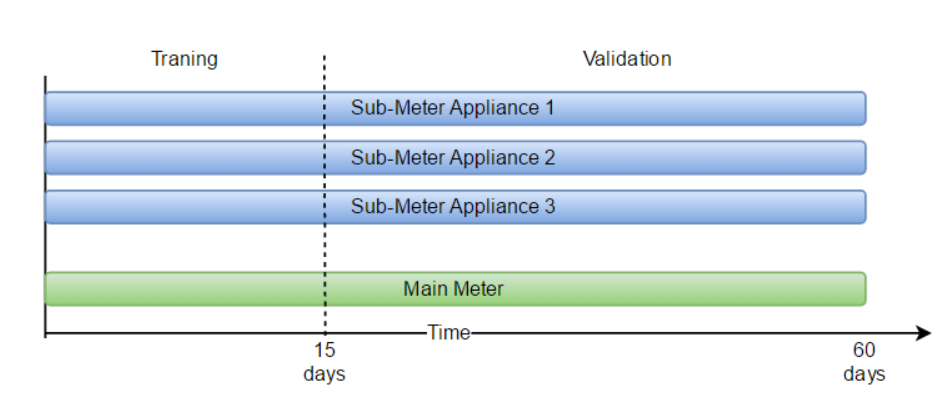
\includegraphics[width=1\textwidth]{billeder/REAL.png}
\caption{Disaggregation phases}
\label{fig:IDF}
\end{figure}

All experiments conducted in the chapter will start with a training phase of 15 days. During this period the sub-meter and main meter data will be used to by the \ab{FHMM} and Parson algorithm to learn statistical disaggregation models. After this initial training phase will the algorithms be tasked with the job of disaggregating the main meter signal in a 45 day validation period. The algorithms will only have access to the data supplied by the main meter, and the statistical disaggregation models found in the initial training phase. The sub-meter data in the validation phase be used to validate the results of the disaggregation. The basis setup is illustrated in figure \ref{fig:IDF} where the green color symbolises data from main meter, and blue symbolises data from sub-meter. 


\section{Challenges In The SmartHG Dataset} 
The \ab{ECO} dataset used in the last chapter, consists of 6 households and the data is sampled at a rate of 1 Hz over a period of 8 months. The SmartHG dataset is different in many aspects. The data is sampled at a slower rate of $\frac{1}{30}$ Hz, but on 25 households over a period of 8 month. Each house have only a small number of sub-meters. The sub-meters are mainly placed on little consumers such as televisions and stereos, which presents an interesting challenge for load disaggregation. The SmartHG dataset contains both the accumulated power, and the instantaneous power usages of the different households.

\begin{figure}[H]
\centering
\includegraphics[width=1\textwidth]{billeder/TotalPie.png}
\caption{Energy distribution in a household}
\label{fig:SLC}
\end{figure}

The power distribution of three households is shown in figure \ref{fig:SLC}. This illustrates how much energy each appliance uses, in relation to the households total energy consumption. The "other" category shows the energy consumption not accounted for by the sub-meters.  

Household 3,10 and 18 are some of the houses that have the smallest \df{other} category. They are therefore selected for further study, since they provide the most information about the house. For the energy distribution in the other households in the SmartHG dataset see Appendix~\ref{APP:AllH}. 

\section{Background Consumption Influence On Disaggregation}
\label{sec:AppNoise}
The households in the SmartHG dataset have a relative big consumption created by appliances in the \df{other} category. The consumption in the \df{other} category is created by appliances that are unknown. In order to do disaggregation, statistical models like models based on the \ab{FHMM} and Parson algorithms, must first be created. This requires knowledge about the appliances consumption. This kind of information is not available for appliances in the \df{other} category. 

This consumption created by appliances that is not part of the statistical disaggregation models can be thought of as "background consumption". The appliances in the \df{other} category will always create \df{background consumption}. This does not exclude appliances that are not part of the \df{other} category from creating \df{background consumption}. All appliances that are not part of the statistical disaggregation models, contribute to the \df{background consumption}.

\subsection{Detection In An Environment With High Background Consumption}
\label{sec:NOISE}
To investigate the influence \df{background consumption} have on a \ab{NILM} application, disaggregation of the known appliances of house 3, 10 and 18 are done using the Parson and \ab{FHMM} algorithms. 

\begin{table}[H]                             
\centering                                   
\begin{tabular}{cc|c|c|c|c|}
\cline{3-6}
\multicolumn{1}{l}{}                            &        & \multicolumn{2}{c|}{FHMM} & \multicolumn{2}{c|}{Parson} \\ \cline{3-6} 
\multicolumn{1}{l}{}                            &        & F1        & Accuracy      & F1         & Accuracy       \\ \hline
\multicolumn{1}{|c|}{\multirow{3}{*}{House 3}}  & TV 1   & 0.19      & 0.74          & 0.10       & 0.40           \\ \cline{2-6} 
\multicolumn{1}{|c|}{}                          & PC     & 0.19      & 0.84          & 0.13       & 0.45           \\ \cline{2-6} 
\multicolumn{1}{|c|}{}                          & TV 2   & 0.03      & 0.84          & 0.20       & 0.11           \\ \hline
\multicolumn{1}{|c|}{\multirow{4}{*}{House 10}} & TV 1   & 0.60      & 0.76          & 0.40       & 0.25           \\ \cline{2-6} 
\multicolumn{1}{|c|}{}                          & Stereo & -         & 1.00          & -          & 1.00           \\ \cline{2-6} 
\multicolumn{1}{|c|}{}                          & PC     & -         & 0.99          & -          & 0.99           \\ \cline{2-6} 
\multicolumn{1}{|c|}{}                          & TV 2   & -         & 0.99          & -          & 0.99           \\ \hline
\multicolumn{1}{|c|}{\multirow{3}{*}{House 18}} & TV 1   & 0.36      & 0.65          & 0.24       & 0.14           \\ \cline{2-6} 
\multicolumn{1}{|c|}{}                          & Lamp   & -         & 0.99          & -          & -              \\ \cline{2-6} 
\multicolumn{1}{|c|}{}                          & TV 2   & 0.73      & 0.58          & -          & 0.00           \\ \hline
\end{tabular}                               
\caption{Appliance disaggregation results of house 3,10 and 18 for the SmartHG dataset.}                     
\label{table:Tab:SHGREAL}                    
\end{table}                   

As previously stated is the \df{background consumption} high for this dataset. Table \ref{table:Tab:SHGREAL} summarizes the results from the disaggregation. The low F1 scores indicates that it is hard for the algorithms to correctly disaggregate the meters. This is due to the many spikes there are in the data that can indicate a change in appliance usage. In figure \ref{fig:RMD} is a snippet from the validation period shown. The blue lines shows the data as it is received from the smart-meter. The other lines indicates the appliances. In the sub plot named "True Signals", on the left side, is the true consumption shown for all the meters. This consumption is known from the sub-meters on the appliances. In the sub plot named "Inferred Signal", on the right, side is the inferred usages of the different appliances created by the \ab{FHMM} algorithm. 

\begin{figure}[H]
\begin{picture}(0,150)
\put(0,10){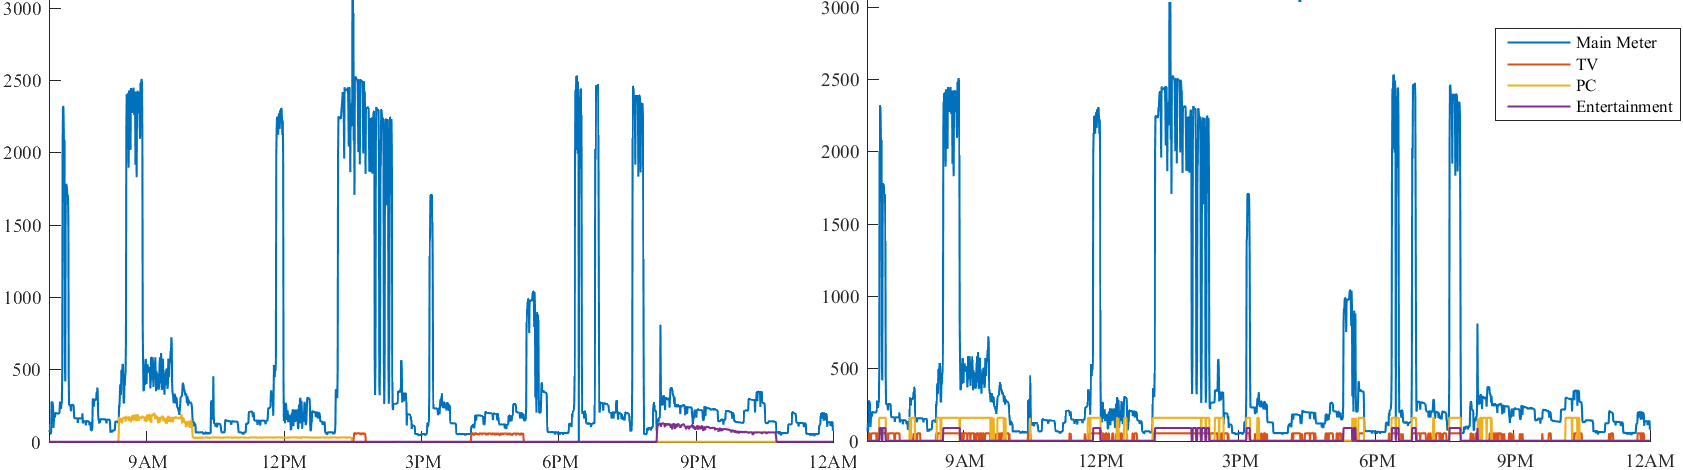
\includegraphics[width=1\textwidth]{billeder/RecognitionEx1.png}}

\put(90,140){True Signals}
\put(300,140){Inferred Signal}

\put(-10,65){\rotatebox{90}{Watt}}
\put(215,0){Time}

\end{picture}
\caption{FHMM disaggregation snippet}
\label{fig:RMD}
\end{figure}

In the figure does the blue lines illustrates how the main meter have many fluctuations. The algorithm tries to map each fluctuation to a change in an appliance state, or as \df{background consumption}. There are many of the fluctuations created by the \df{background consumption} that are similar to the power changes created by the TV, PC and entertainment system. The inferred signal shows how the algorithm thinks the appliances is used. It is easily seen that this is quite different from the true values. 

\subsection{Detection In An Environment With No Background Consumption}
\label{sec:NOISEFREE}
The assumption that the \df{background consumption} is what troubles the disaggregation dictates that for a house where all appliances are known, and there are no \df{background consumption}, the disaggregation will perform better. 

\begin{figure}[H]
\centering
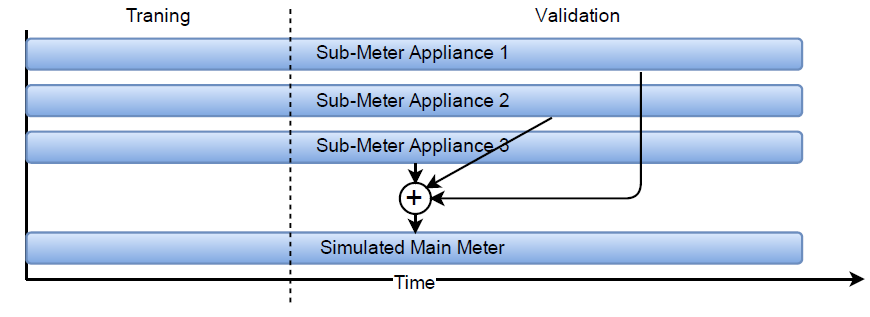
\includegraphics[width=1\textwidth]{billeder/SimIllu.png}
\caption{Artificially constructed main meter}
\label{fig:SIL}
\end{figure}

In order to test this hypothesis is a main meter signal artificially constructed by summing the values of all the sub-meters in a house. This process is illustrated in figure \ref{fig:SIL}. In this manner is a new set of artificial houses created where there are no \df{background consumption}. By applying the same disaggregation algorithms, as for the environment with high \df{background consumption}, on the new environment with no \df{background consumption} is the performance much increased as shown in table \ref{table:Tab:SHGSIM}.

\begin{table}[H]                             
\centering                                   
\begin{tabular}{cc|c|c|c|c|}
\cline{3-6}
                                                &        & \multicolumn{2}{c|}{FHMM} & \multicolumn{2}{c|}{Parson} \\ \cline{3-6} 
                                                &        & F1        & Accuracy      & F1         & Accuracy       \\ \hline
\multicolumn{1}{|c|}{\multirow{3}{*}{House 3}}  & TV 1   & 0.73      & 0.96          & 0.26       & 0.86           \\ \cline{2-6} 
\multicolumn{1}{|c|}{}                          & PC     & 0.74      & 0.96          & 0.30       & 0.91           \\ \cline{2-6} 
\multicolumn{1}{|c|}{}                          & TV 2   & 0.83      & 0.96          & 0.20       & 0.11           \\ \hline
\multicolumn{1}{|c|}{\multirow{4}{*}{House 10}} & TV 1   & 0.97      & 0.98          & 0.40       & 0.25           \\ \cline{2-6} 
\multicolumn{1}{|c|}{}                          & Stereo & -         & 1.00          & -          & 1.00           \\ \cline{2-6} 
\multicolumn{1}{|c|}{}                          & PC     & -         & 0.99          & -          & 0.99           \\ \cline{2-6} 
\multicolumn{1}{|c|}{}                          & TV 2   & -         & 0.99          & -          & 0.99           \\ \hline
\multicolumn{1}{|c|}{\multirow{3}{*}{House 18}} & TV 1   & 0.95      & 0.98          & 0.24       & 0.14           \\ \cline{2-6} 
\multicolumn{1}{|c|}{}                          & Lamp   & -         & 0.99          & -          & -              \\ \cline{2-6} 
\multicolumn{1}{|c|}{}                          & TV 2   & 0.73      & 0.58          & 0.73       & 0.58           \\ \hline
\end{tabular}                              
\caption{Disaggregation of appliances on artificially constructed main meters }                     
\label{table:Tab:SHGSIM}                     
\end{table}   

The F1 and accuracy score are both improve, as shown in table \ref{table:Tab:SHGSIM}. Even though the artificial house only contains three or four appliances, and all are accounted for by the statistical disaggregation model created by the \ab{FHMM} and Parson algorithms, there are still some of the appliances that are hard to find. This is due to the appliances power usage pattern in OFF/standby mode combined with the rare usage of the devices. When the standby pattern of a device is complex and the appliance is only rarely used the model will try to fit to the standby pattern and not the usage pattern. This happens if the over all best consumption disaggregation results is achieved by fitting to the small energy fluctuations in the OFF state. This is often the case for appliances that are rarely used int the training period. The downside to this is that it will be incapable of detecting change between the ON/OFF states.

One other aspect to note is that even though the F1 scores are higher, only a few is higher than 0.9. 
This could be due to "appliance interference". This happens when appliances are similar. When a house contains two or more appliances that are similar it gets harder for the algorithm to tell if it is the one or the other. This is could be what happened for TV 1 and TV 2 in house 3. The algorithms will wrongfully assign some of the events belonging to TV 1, to TV 2 and vice versa. This happens because the power draw signature are similar.  This can be a problem if the goal is to determine exactly which appliance there is responsible for the power consumption. This is one of the key aspects of the little consumers problem, discussed in Chapter \ref{sec:AppRec}.

\df{Appliance interference} has a profound effect on the Parson algorithm. The parson algorithm is designed to split up appliances based on appliance categories, by utilizing a set of general models. Since a lot of the appliances are similar in their consumption changes from state to state are the model used by the Parson algorithm almost identical which lead to the events being wrongly categorised. The usages general models is one of the benefits of the Parson algorithm, since it makes the algorithm very portable between unknown domains. Unfortunately does this feature come whit the downside of increased sensibility to \df{appliance interference}. The influence of \df{appliance interference} is further studied in Section \ref{sec:MCT}. 

\subsection{Background Consumption Effect On Training And Validation }
The experiments in the two previous Sections \ref{sec:NOISE} and \ref{sec:NOISEFREE} suggest that \df{background consumption} has an impact on the performance of the system. But for a system based on machine learning techniques like the \ab{FHMM} and the Parson algorithms it raises the questions, is it to hard for the system to train the correct statistical disaggregation models in the signal with much \df{background consumption}, or are the \df{background consumption} just interfering with the disaggregation process? 

\begin{figure}[H]
\centering
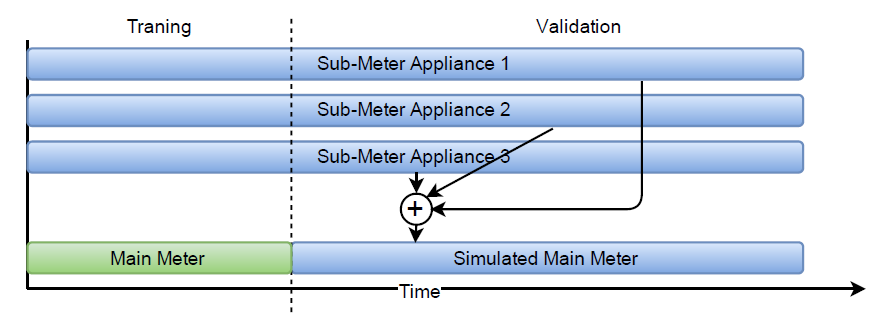
\includegraphics[width=1\textwidth]{billeder/REALSIM.png}
\caption{Illustration of dataset creation by combining real and constructed data}
\label{fig:REALSIMILU}
\end{figure}

In order to investigate these questions was a new dataset created that combined real data collected from the house main meter, and an artificially constructed main meter. The new dataset was created by using the real data in the training period of the house, and constructed main meter data in the validation, as illustrated on figure \ref{fig:REALSIMILU}.

This creates a environment with a lot of \df{background consumption} in the training phase and no \df{background consumption} in the validation phase. If the \df{background consumption} did not influence the creation of the statistical disaggregation models that represent each appliance, then the results were expected to be just as good as for the noise free experiments conducted in Section \ref{sec:NOISEFREE}.


\begin{table}[H]                             
\centering                                   
\begin{tabular}{cc|c|c|c|c|}
\cline{3-6}
\multicolumn{1}{l}{}                            &        & \multicolumn{2}{c|}{FHMM} & \multicolumn{2}{c|}{Parson} \\ \cline{3-6} 
\multicolumn{1}{l}{}                            &        & F1        & Accuracy      & F1         & Accuracy       \\ \hline
\multicolumn{1}{|c|}{\multirow{3}{*}{House 3}}  & TV 1   & 0.20      & 0.94          & 0.23       & 0.86           \\ \cline{2-6} 
\multicolumn{1}{|c|}{}                          & PC     & 0.29      & 0.94          & 0.32       & 0.92           \\ \cline{2-6} 
\multicolumn{1}{|c|}{}                          & TV 2   & 0.00      & 0.88          & 0.20       & 0.11           \\ \hline
\multicolumn{1}{|c|}{\multirow{4}{*}{House 10}} & TV 1   & 0.10      & 0.74          & 0.40       & 0.25           \\ \cline{2-6} 
\multicolumn{1}{|c|}{}                          & Stereo & -         & 1.00          & -          & 1.00           \\ \cline{2-6} 
\multicolumn{1}{|c|}{}                          & PC     & -         & 0.99          & -          & 0.99           \\ \cline{2-6} 
\multicolumn{1}{|c|}{}                          & TV 2   & -         & 0.99          & -          & 0.99           \\ \hline
\multicolumn{1}{|c|}{\multirow{3}{*}{House 18}} & TV 1   & 0.00      & 0.86          & 0.24       & 0.14           \\ \cline{2-6} 
\multicolumn{1}{|c|}{}                          & Lamp   & -         & 0.99          & -          & -              \\ \cline{2-6} 
\multicolumn{1}{|c|}{}                          & TV 2   & 0.73      & 0.58          & 0.73       & 0.58           \\ \hline
\end{tabular}                                
\caption{Disaggregation in real and constructed main meters combined.}                     
\label{table:Tab:SHGREALSIM}                 
\end{table}    

If the results from the experiment, shown in table \ref{table:Tab:SHGREALSIM}, is compared with the results from table \ref{table:Tab:SHGSIM} from section \ref{sec:NOISEFREE} it is clearly seen that the performance of the system trained in real data is much lower than the one trained on artificially constructed data. This indicates that the disaggregation models obtained in the real data is influenced by the \df{background consumption}, and is therefore not fitting accurately enough to the true disaggregation models. This indicates that the low performance in the real data shown in table \ref{table:Tab:SHGREAL} in section \ref{sec:NOISE} is caused by the models not fitting correctly to the true values, and not by the models being triggered by application noise from other appliances.

In order to validate this hypothesis was a similar experiment conducted, where the training data was artificially constructed, and the validation data was the real data from the main meter as illustrated in figure \ref{fig:SHGSIMREAL}. 

\begin{figure}[H]
\centering
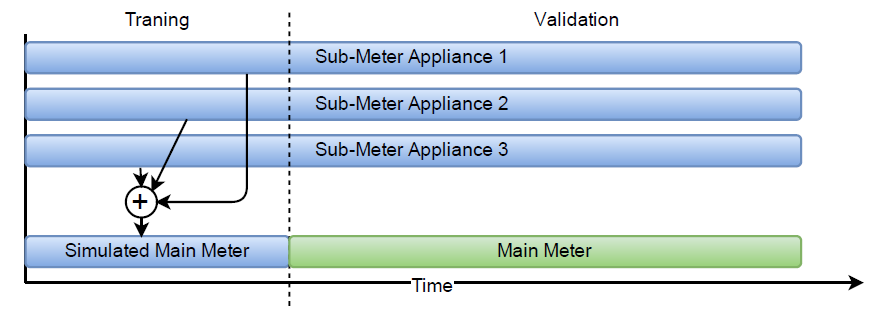
\includegraphics[width=0.9\textwidth]{billeder/SIMREAL.png}
\caption{Illustration of dataset creation by combining constructed and real data}
\label{fig:SHGSIMREAL}
\end{figure}

By training the model on the constructed data, is the true model for the appliances more easily found. If the environment with high \df{background consumption} and real data is non-interfering with the disaggregation models can a performance like for the artificially constructed environment, with no \df{background consumption}, described in Section \ref{sec:NOISEFREE} be expected for the validation phase. 


\begin{table}[H]                             
\centering                                   
\begin{tabular}{lc|c|c|c|c|}
\cline{3-6}
                                                &        & \multicolumn{2}{c|}{FHMM} & \multicolumn{2}{c|}{Parson} \\ \cline{3-6} 
                                                &        & F1        & Accuracy      & F1         & Accuracy       \\ \hline
\multicolumn{1}{|l|}{\multirow{3}{*}{House 3}}  & TV 1   & 0.10      & 0.42          & 0.10       & 0.45           \\ \cline{2-6} 
\multicolumn{1}{|l|}{}                          & PC     & 0.13      & 0.39          & 0.12       & 0.44           \\ \cline{2-6} 
\multicolumn{1}{|l|}{}                          & TV 2   & 0.21      & 0.35          & 0.20       & 0.11           \\ \hline
\multicolumn{1}{|l|}{\multirow{4}{*}{House 10}} & TV 1   & 0.40      & 0.25          & 0.40       & 0.25           \\ \cline{2-6} 
\multicolumn{1}{|l|}{}                          & Stereo & -         & 1.00          & -          & 1.00           \\ \cline{2-6} 
\multicolumn{1}{|l|}{}                          & PC     & -         & 0.99          & -          & 0.99           \\ \cline{2-6} 
\multicolumn{1}{|l|}{}                          & TV 2   & -         & 0.99          & -          & 0.99           \\ \hline
\multicolumn{1}{|l|}{\multirow{3}{*}{House 18}} & TV 1   & 0.27      & 0.26          & 0.24       & 0.14           \\ \cline{2-6} 
\multicolumn{1}{|l|}{}                          & Lamp   & -         & 0.99          & -          & -              \\ \cline{2-6} 
\multicolumn{1}{|l|}{}                          & TV 2   & 0.73      & 0.58          & 0.73       & 0.58           \\ \hline
\end{tabular}                              
\caption{Disaggregation in constructed and real main meters combined}                     
\label{table:Tab:SHGSIMREAL}                 
\end{table}     

The results are shown in table \ref{table:Tab:SHGSIMREAL}. The performance of this experiment is lower than for the one in the environment with no \df{background consumption}. This lead to the conclusion that the \df{background consumption} is both affecting the models, and interfering in the validation process.  

The results from the disaggregation of the data in the real environment from section \ref{sec:NOISE} are compared with the results from the the previous experiments, where the models were extracted from constructed data and validated on the real data. The results is summarized in table \ref{table:Tab:RealVsCon}. 

\begin{table}[H]                             
\centering                                   
\begin{tabular}{ccccccc}
\cline{3-4} \cline{6-7}
\multicolumn{1}{l}{}                            & \multicolumn{1}{c|}{}       & \multicolumn{2}{c|}{FHMM}                                 & \multicolumn{1}{c|}{} & \multicolumn{2}{c|}{FHMM}                                 \\
\multicolumn{1}{l}{}                            & \multicolumn{1}{c|}{}       & \multicolumn{2}{c|}{Real}                                 & \multicolumn{1}{c|}{} & \multicolumn{2}{c|}{Constructed}                          \\ \cline{3-4} \cline{6-7} 
\multicolumn{1}{l}{}                            & \multicolumn{1}{c|}{}       & \multicolumn{1}{c|}{F1}   & \multicolumn{1}{c|}{Accuracy} & \multicolumn{1}{c|}{} & \multicolumn{1}{c|}{F1}   & \multicolumn{1}{c|}{Accuracy} \\ \cline{1-4} \cline{6-7} 
\multicolumn{1}{|c|}{\multirow{3}{*}{House 3}}  & \multicolumn{1}{c|}{TV 1}   & \multicolumn{1}{c|}{0.19} & \multicolumn{1}{c|}{0.74}     & \multicolumn{1}{c|}{} & \multicolumn{1}{c|}{0.10} & \multicolumn{1}{c|}{0.42}     \\ \cline{2-4} \cline{6-7} 
\multicolumn{1}{|c|}{}                          & \multicolumn{1}{c|}{PC}     & \multicolumn{1}{c|}{0.19} & \multicolumn{1}{c|}{0.84}     & \multicolumn{1}{c|}{} & \multicolumn{1}{c|}{0.13} & \multicolumn{1}{c|}{0.39}     \\ \cline{2-4} \cline{6-7} 
\multicolumn{1}{|c|}{}                          & \multicolumn{1}{c|}{TV 2}   & \multicolumn{1}{c|}{0.03} & \multicolumn{1}{c|}{0.84}     & \multicolumn{1}{c|}{} & \multicolumn{1}{c|}{0.21} & \multicolumn{1}{c|}{0.35}     \\ \cline{1-4} \cline{6-7} 
\multicolumn{1}{l}{}                            &                             &                           &                               &                       &                           &                               \\ \cline{1-4} \cline{6-7} 
\multicolumn{1}{|c|}{\multirow{4}{*}{House 10}} & \multicolumn{1}{c|}{TV 1}   & \multicolumn{1}{c|}{0.60} & \multicolumn{1}{c|}{0.76}     & \multicolumn{1}{c|}{} & \multicolumn{1}{c|}{0.40} & \multicolumn{1}{c|}{0.25}     \\ \cline{2-4} \cline{6-7} 
\multicolumn{1}{|c|}{}                          & \multicolumn{1}{c|}{Stereo} & \multicolumn{1}{c|}{-}    & \multicolumn{1}{c|}{1.00}     & \multicolumn{1}{c|}{} & \multicolumn{1}{c|}{-}    & \multicolumn{1}{c|}{1.00}     \\ \cline{2-4} \cline{6-7} 
\multicolumn{1}{|c|}{}                          & \multicolumn{1}{c|}{PC}     & \multicolumn{1}{c|}{-}    & \multicolumn{1}{c|}{0.99}     & \multicolumn{1}{c|}{} & \multicolumn{1}{c|}{-}    & \multicolumn{1}{c|}{0.99}     \\ \cline{2-4} \cline{6-7} 
\multicolumn{1}{|c|}{}                          & \multicolumn{1}{c|}{TV 2}   & \multicolumn{1}{c|}{-}    & \multicolumn{1}{c|}{0.99}     & \multicolumn{1}{c|}{} & \multicolumn{1}{c|}{-}    & \multicolumn{1}{c|}{0.99}     \\ \cline{1-4} \cline{6-7} 
\multicolumn{1}{l}{}                            &                             &                           &                               &                       &                           &                               \\ \cline{1-4} \cline{6-7} 
\multicolumn{1}{|c|}{\multirow{3}{*}{House 18}} & \multicolumn{1}{c|}{TV 1}   & \multicolumn{1}{c|}{0.36} & \multicolumn{1}{c|}{0.65}     & \multicolumn{1}{c|}{} & \multicolumn{1}{c|}{0.27} & \multicolumn{1}{c|}{0.26}     \\ \cline{2-4} \cline{6-7} 
\multicolumn{1}{|c|}{}                          & \multicolumn{1}{c|}{Lamp}   & \multicolumn{1}{c|}{-}    & \multicolumn{1}{c|}{0.99}     & \multicolumn{1}{c|}{} & \multicolumn{1}{c|}{-}    & \multicolumn{1}{c|}{0.99}     \\ \cline{2-4} \cline{6-7} 
\multicolumn{1}{|c|}{}                          & \multicolumn{1}{c|}{TV 2}   & \multicolumn{1}{c|}{0.73} & \multicolumn{1}{c|}{0.58}     & \multicolumn{1}{c|}{} & \multicolumn{1}{c|}{0.73} & \multicolumn{1}{c|}{0.58}     \\ \cline{1-4} \cline{6-7} 
\end{tabular}                         
\caption{Trained in real vs. constructed data}                     
\label{table:Tab:RealVsCon}                    
\end{table}  

The table shows that the performance of the system is better when trained in the real environment, as in relation to when the the system is trained in a artificial environment and then deployed in a environment with \df{background consumption}. This is in contrast to what one might think, since the environment with no \df{background consumption} should have supplied more correct models. But when the \df{background consumption} is removed from a house, in the training process, is a offset error introduced in the models. 

Appliances such as refrigerators and freezers that are always on will create a local house offset. This will vary from house to house, and is depended on the types and number of appliances in the house. If only a small number of devices are modelled in each house, as in the SmartHG case, is the offset almost exclusivity a part of the \df{background consumption}. When the models are learned in the training phase in the real data, is the offset learned into the model, and further improves the model. This is not the case when the model are trained in the constructed dataset. 

If not all appliances in a house are known, a better performance can therefore be obtained by training in the intended environment of deployment. 

Some algorithms are designed to not be affected by the house offset, and is therefore moved from different environments more easily. The Parson algorithm is designed with this in mind. The performance of the Parson algorithm is therefore the same, or in some cases improved, when using models trained in constructed data. This advantage unfortunately comes with the problem of generalization, which lead to harder source separation, as discussed in section \ref{sec:NOISE}. 

\subsection{Improving Performance Using Norm Knowledge }
\label{sec:NormFilter}
When an appliance is in a environment with a lot of \df{background consumption} some of the \df{background consumption} can be interpreted as the appliance.This \df{appliance interference} creates a scenario where it seems like the appliance is used more than it actually is. Often does the \df{appliance interference} create usage patterns that is in contrast to that one would expect. This can make it seems like a appliance is used in a unrealistic manner. By improving the method with the knowledge of how a specific appliance is most commonly used, also called the norm usage, it is possible to filter the signal and improve the performance. 

In figure \ref{fig:Norm1} is the disaggregation of TV 1 from house 10 shown for an one day period. The blue line indicate the \ab{FHMM} algorithms suggestions on when the TV are ON and OFF. The green line is the actual ON and OFF periods, collected from the sub-meters. 

\begin{figure}[H]
\centering
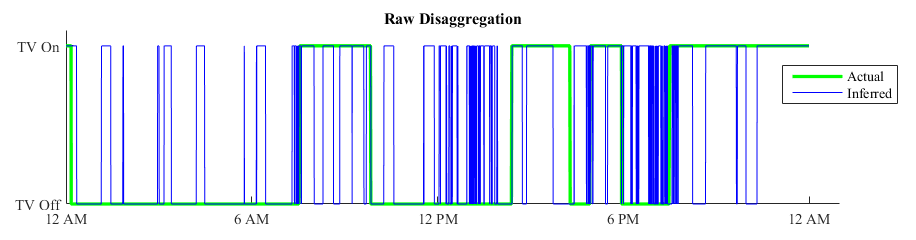
\includegraphics[width=1\textwidth]{billeder/AppNormFilterH10_1.png}
\caption{Disaggregation of TV 1 from house 10}
\label{fig:Norm1}
\end{figure}

As seen in the figure there is a lot of small spikes that are less than 10 min, and sometime is the TV ON for 15 minutes off in 2 and then on again for another 15 minutes. This behaviour does not fit the normal behaviour one would expect for a person. The norm is to see TV more than 20 minutes of the time, and when a TV is turned off it is common that it is turned off for atleast 15 minutes before turned on again. These numbers are a loose estimate, found by observing the sub-meter data. 

%% Rettelser til dette punkt - (Mangler stadig tabeller!!) 

One approach of applying the norm knowledge to the disaggregation result is to use a "Norm filter". This is a filter that takes the results from the disaggregation and removes unrealistic behaviour. This is achieved by using a method that iteratively purges events from the signal and merges events that are too close to one event. The "purge and merge process" runs two iterations. First is all events shorter than 10 minutes are purged from the signal.Next is events separated with less than 15 minutes of off time are merged. The purge and merge cycle is repeated one more time where events shorter than 25 minutes are purged and events closer than 30 min are merged. 

The values used in the \df{purge and merge process} is found experimentally. These parameters gave the best results for the TV's in the experiments. In a real deployment scenario where a \df{norm filter} was applied, the coefficients must be selected to fit the normal behaviour of the residents.

The downside of this approach is that it assumes that the devices is used in a certain manner. For our example of values found for a TV will all watch sessions shorter than 25 minutes be missed.

\begin{figure}[H]
\centering
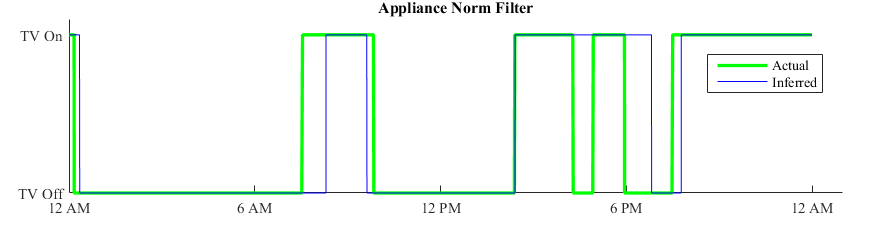
\includegraphics[width=1\textwidth]{billeder/AppNormFilterH10_2.png}
\caption{Purged and merged signal from TV 1}
\label{fig:Norm2}
\end{figure}

In figure \ref{fig:Norm2} is the same signal as in figure \ref{fig:Norm1} filtered by using the \df{norm filter}. As seen in figure \ref{fig:Norm2} does the signal inferred by the filtered \ab{FHMM} algorithm match more closely to the actual signal. 

In this example is the norm knowledge applied as a filter, that can filter the disaggregation result. Another approach could be to integrate the norm knowledge as a component in the state transition probability of the \ab{HMM}.

The \df{Norm filter} is only recommended if the accuracy and F1 score of the disaggregation is low. It is undesirable to force the system to enforce the normal usage as the truth. This can filter away accentually events, that lay outside the norm. But for systems that have a low accuracy and F1 score can this approach help clean the signal. 

\section{Model Complexity And Completeness Influence }
\label{sec:MCACI}
Some of the parameters that often differ in the environments where\ab{NILM} applications are deployed, is the number of appliances. As previously disused is not all appliances included in the statistical disaggregation models used by the \ab{FHMM} and Parson algorithms. These are the appliances creating the \df{background consumption}. The statistical disaggregation models often contain the information needed to do disaggregation on multiple appliances. The number of appliances included in the statistical disaggregation model is defined as the "complexity" of the model. The \df{complexity} tells only how many appliances a given model is trained to detect. As the \df{complexity} in a \ab{NILM} application is increasing the detection rate is deceasing~\citep{RefWorks:34}. This is one of the major problems and is why many researchers only focus on a small subset of appliances that have a fairly unique consumption signature. The \df{complexity} tells nothing about the appliances creating the \df{background consumption}. 

An other metric looks at the ratio between the \df{complexity} and the total number of appliances in the environment. This ratio is called the "completeness" of the model, since it indicate how many of the total appliances that are include in the model. The total number of appliances in the environment can be seen as the number of appliances creating the \df{background consumption} plus the \df{complexity}.


\subsection{Test Set Creation}
\label{sec:datasetCreation}
In order to experiment with the \df{completeness} and \df{complexity} of the statistical disaggregation models in the SmartHG dataset is a more controllable environment required. In order to obtain this is a series of datasets artificially constructed from the SmartHG dataset. 

First an artificial house dataset where created called the "TV House dataset". The \df{TV house dataset} is created by picking the relative dominant TV signals from the houses 5, 10, 11, 13, 18 and 23 in the SmartHG dataset. By combining the signals to one artificial signal can a artificial main meter for a house with 7 TV's be created. 

The \df{TV House dataset} consists of dominant appliances, and there is no \df{background consumption} from unknown devices. It is still worth noticing that all the 7 appliances are a Type-II appliances, and they are all TV's, which make there usage pattern some what similar. Since the Parson algorithm is greatly effected by this. Therefore will the focus mainly be on the \ab{FHMM} algorithm. 

If the \df{TV House dataset} was seen as a set of sub-meters as mathematically shown in equation \ref{EQ:SUBMS}. Where $TV_n$ is a vector containing the consumption data collected for a specific TV.

\begin{equation}
	\textbf{S}_{full} = \{ TV_1, TV_2, ... , TV_7 \}
	\label{EQ:SUBMS}
\end{equation}

Since there is no \df{background consumption}, can the main meter data be artificially created as the sum of sub-meters data as shown in equation \ref{EQ:SUMSUB}. Where $X$ is the vector of sub-meter measurements from the televisions. $M_{main}$ is a vector containing the artificial main meter consumption data. 

\begin{equation}
	M_{main} = \sum_{X \in \textbf{S}_{full}}X
	\label{EQ:SUMSUB}
\end{equation}

Using this approach it is possible to create a set with a specific number of appliances. This can be achieved by taking a subset of the $\textbf{S}_{full}$ set with the cardinality of the desired number of appliances. The main meter can now be found for this subset, using the same principle as in equation \ref{EQ:SUMSUB}. Using the equation \ref{EQ:TVCARSET}, it is possible to find a set of all sets with a desired number of appliances $c$.

\begin{equation}
	\textbf{H}_c = \{ x | x \in \powerset{\textbf{S}_{full}}, \forall |x| = c   \}
	\label{EQ:TVCARSET}
\end{equation}

This is done using a set comprehension that iterates over the power set of $\textbf{S}_{full}$ and picking out all sets that have a cardinality equal to the desired number of appliances $c$. $\textbf{H}_c$ is therefore a set of sets with a given number of appliances. This can be graphically shown as in figure \ref{fig:PSILLU}. 

\begin{figure}[H]
\begin{picture}(0,200)
\put(0,0){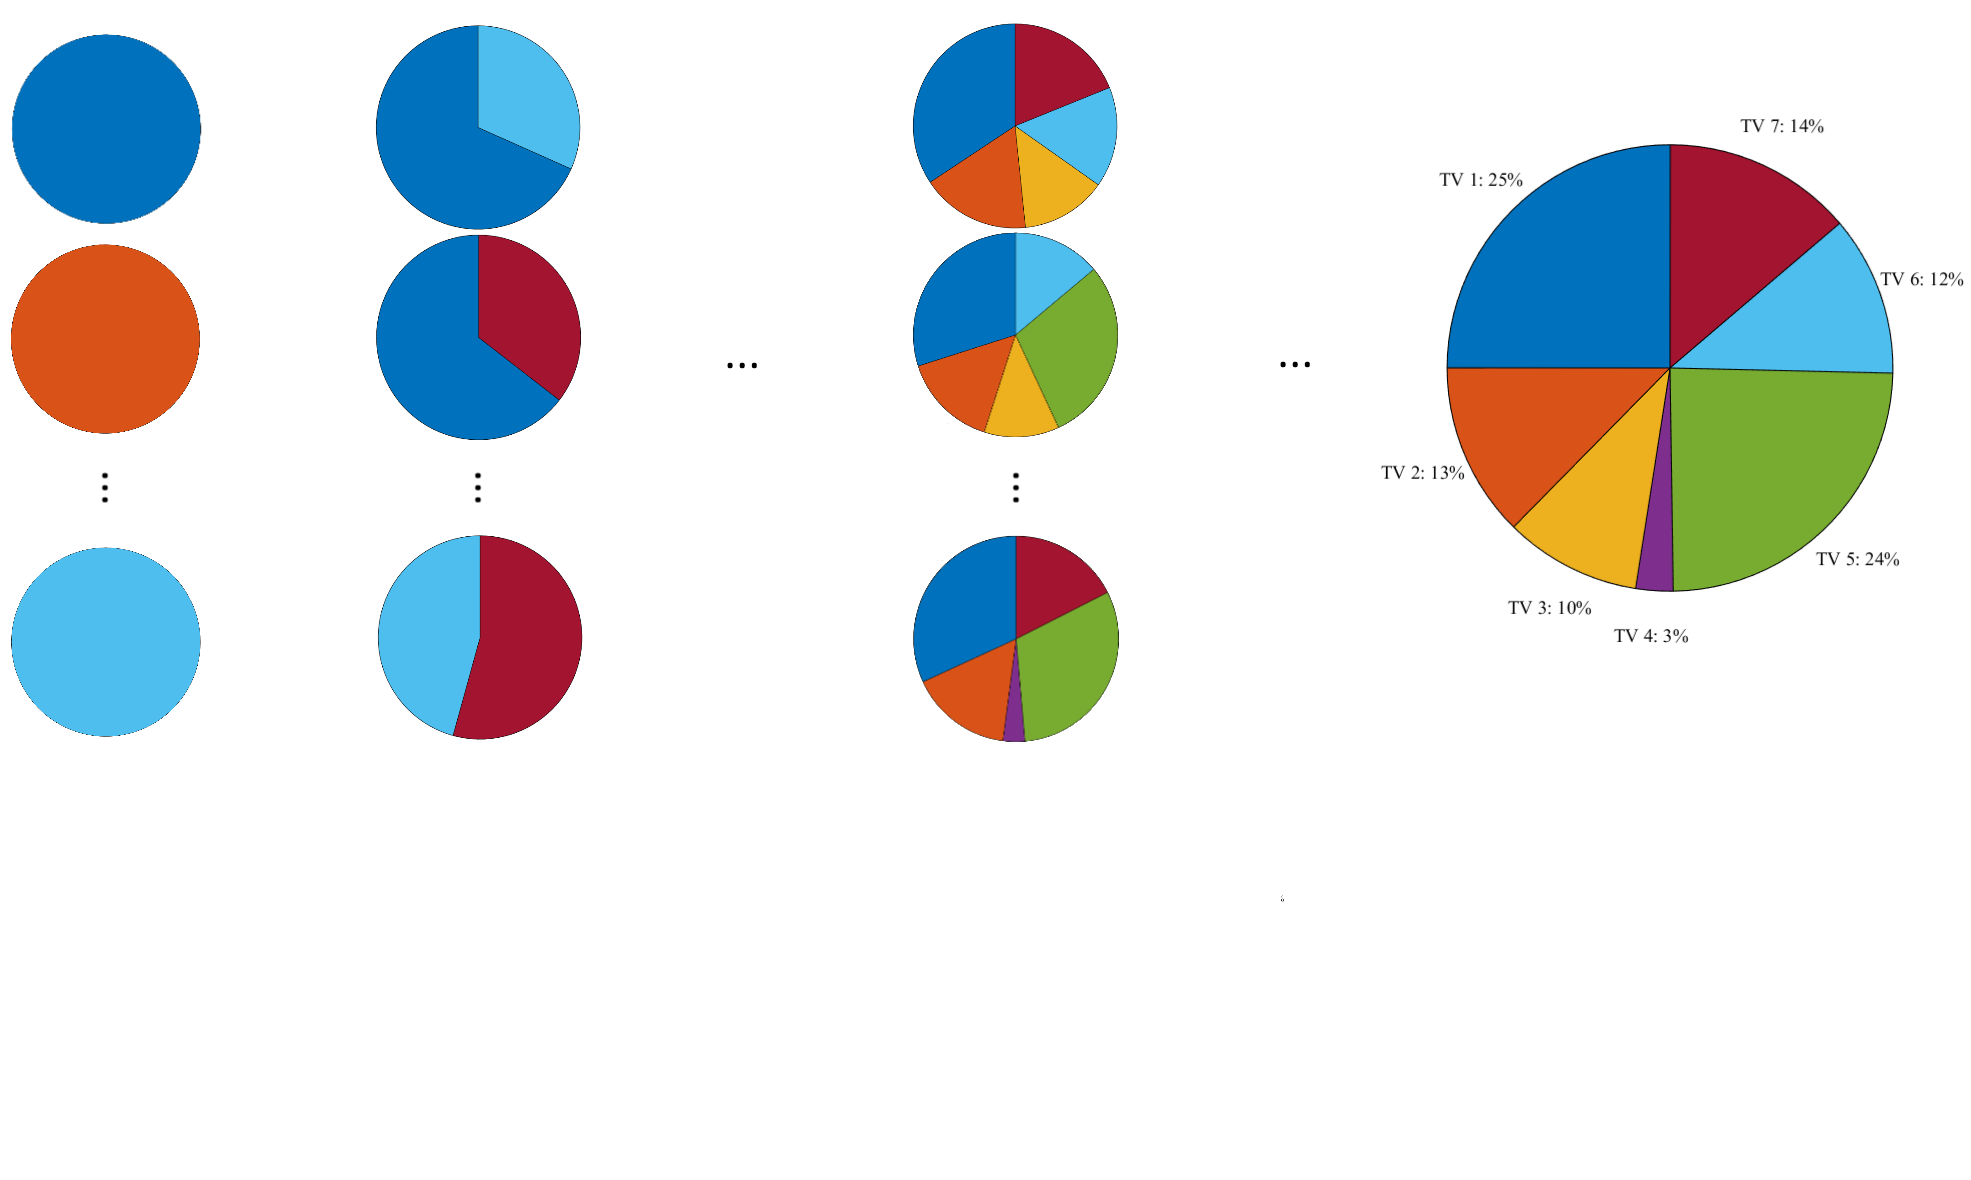
\includegraphics[width=1\textwidth]{billeder/CombiShow.png}}

\put(20,10){$\textbf{H}_1$}
\put(105,10){$\textbf{H}_2$}
\put(230,10){$\textbf{H}_5$}
\put(375,10){$\textbf{H}_7$}

\end{picture}
\caption{$\textbf{H}_c$ sets from the TV house dataset}
\label{fig:PSILLU}
\end{figure}

Where the $\textbf{H}_7$ only contains the $\textbf{S}_{full}$ set. In the figure is illustrated the relative energy usage of each appliance in a dataset.   In this manner it is possible to artificially create one or more datasets with a desired number of appliances, equal to or less than the number of appliances in $\textbf{S}_{full}$. The amount of artificiality created houses for a desired number of appliances can be found by using the simple combinatorial equation shown in equation \ref{EQ:nCr}. Where $|\textbf{H}_c|$ is the cardinality of $\textbf{H}_c$. The number of desired appliances is $c$, and the size of the pool for which appliances can be selected from is given by the cardinality of $\textbf{S}_{full}$.

\begin{gather}
		|\textbf{H}_c| = \frac{|\textbf{S}_{full}|!}{c! \times (|\textbf{S}_{full}| - c)!} \label{EQ:nCr} \\
		A_c = |\textbf{H}_c| \times \frac{c}{|\textbf{S}_{full}|} \label{EQ:ACr}
\end{gather}
% n! / ( r! (n - r)! )


As illustrated in figure \ref{fig:PSILLU} can an appliance appear in multiple sets in a given $\textbf{H}_c$ collection. The number of sets containing a specific appliance in a $\textbf{H}_c$ collection is $A_c$. This can be calculated as in equation \ref{EQ:ACr}. In order to ensure that the combination of appliances does not have an effect on the experiments, are the experiments conducted on all combinations in $\textbf{H}_c$. The results for each experiment is an average of the performance for the appliance in the experiment. 

\begin{table}[]
\centering
\begin{tabular}{c|c|c|c|c|c|c|c|}
\cline{2-8}
                       & $c = 1$ & $c = 2$ & $c = 3$ & $c = 4$ & $c = 5$ & $c = 6$ & $c = 7$ \\ \hline
\multicolumn{1}{|c|}{$|\textbf{H}_c|$} &    7   &    21   &    35   &    35   &   21    &   7    &    1  \\ \hline
\multicolumn{1}{|c|}{$A_c$} &    1   &     6  &     15  &     20  &    15   &    6   &    1   \\ \hline
\end{tabular}
\caption{TV House dataset complexity}
\label{Tab:TvHouse}
\end{table}

In the case of the \df{TV house dataset} can the cardinality of $\textbf{H}_c$ and $A_c$ values for the different number of appliances $c$, be seen in table \ref{Tab:TvHouse}. The cardinality of $\textbf{H}_c$ tells how many artificial houses can be constructed with the desired number of appliances $c$. The $A_c$ values tells how many artificial houses contains a specific TV.


\subsection{Model Complexity Test}
\label{sec:MCT}
To investigate the effect the \df{complexity} of the statistical disaggregation models have on the performance of a \ab{NILM} system, is disaggregation done on every artificial house that can be created from $\textbf{H}$. The experiment is conducted by training the models be able to disaggregate all the appliances in a given scenario. This creates an environment where there is no \df{background consumption} that can interfere.

\begin{figure}[H]
\centering
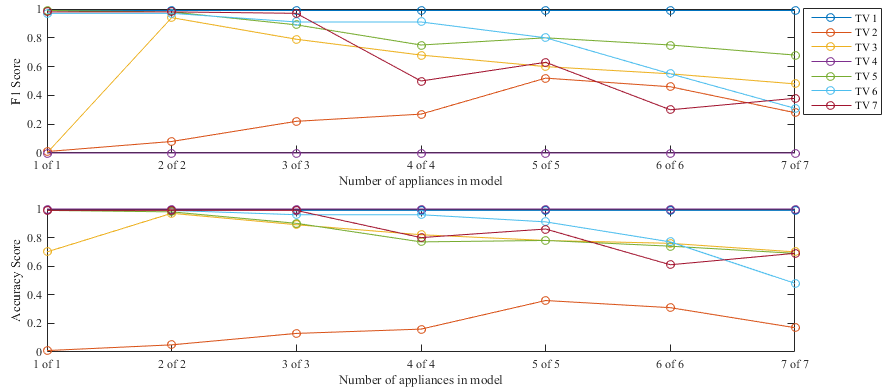
\includegraphics[width=1\textwidth]{billeder/ModelSize.png}
\caption{Average score at different complexity }
\label{fig:COMPT}
\end{figure}

The test is performed on every combination, to ensure that there is not some combination that are more favourable than others. The results shown in figure \ref{fig:COMPT} are the average of the results from the many combinations as described in section \ref{sec:datasetCreation}. 

For the most part it is fairly easy to correctly classify the TV's when the complexity is only one. As a general trend does the F1 and accuracy score of the TV's decrease as the complexity of the house increase. This is due to the \df{Application interference}. The \df{Application interference} effect is when there actually is an event, but the system classifies it to the wrong device.  An effect of this is most clearly seen on TV 2 signal. TV 2 is a very complex signal, and is therefore hard to track by the algorithm, as seen at the $\textbf{H}_1$ complexity that have an F1 score on almost zero. When the complexity is increased it looks like it is easier to detect the signal, and the F1 score is increasing. What is actually happening is \df{Application interference} from the other TV's. Since all the appliances are TV's they have a lot of overlap in their usage. A lot of people watches TV at the same time of day e.g. between 18:00-22:00. This makes the algorithm encounter signal's that are similar in structure for the different TV's. It has a hard time deciding which appliance is responsible. Therefore can some events generated by the other TV's be assigned as TV 2. If by chance TV 2 actually was on when the events from the other TV's was wrongfully assigned, the F1 and accuracy score of TV 2 would improve. 

For other appliances that are not as hard to classify as TV 2 will the \df{appliance interference} effect decrease the F1 and accuracy score as seen in the figure. 

\subsection{Model Completeness Influence }
In the experiments conducted on the the SmartHG dataset in section \ref{sec:AppNoise} it was shown that the \df{appliance interference} made it hard to correctly disaggregate the appliances of the houses. In the last experiment in section \ref{sec:MCT}, it was shown that the performance of the disaggregation was higher when the \df{complexity} of the house was low. This is much the same results as seen in the experiments on the SmartHG dataset. The completely simulated houses that had a low \df{complexity}, preformed better, than the real house with a high \df{complexity}. 

But in the SmartHG dataset was the \df{complexity} of the real dataset unknown since the amount of appliances that generated the \df{background consumption} is unknown. It is therefore hard to conclude if the poor performance in the real data is due to the fact that the appliances is unknown by the disaggregation model, or because the \df{complexity} of the house is greater for the real data. 

To further investigate this was an experiment conducted on the \df{TV house dataset}, where the statistical disaggregation models where trained on the $\textbf{H}_{7}$ dataset. The models trained did not contain the full knowledge of the house. The models was only trained to find a subset of meters in the house. Like for the experiments in section \ref{sec:MCT}, was the experiment conducted on all subset combinations. This creates a test where the amount of \df{background consumption} is artificially controlled. There is a lot of \df{background consumption} when there only is one appliance in the disaggregation model, and non if all seven appliances is in the disaggregation model. This can also be seen as a change in the \df{completeness} of the model. 

\begin{figure}[H]
\centering
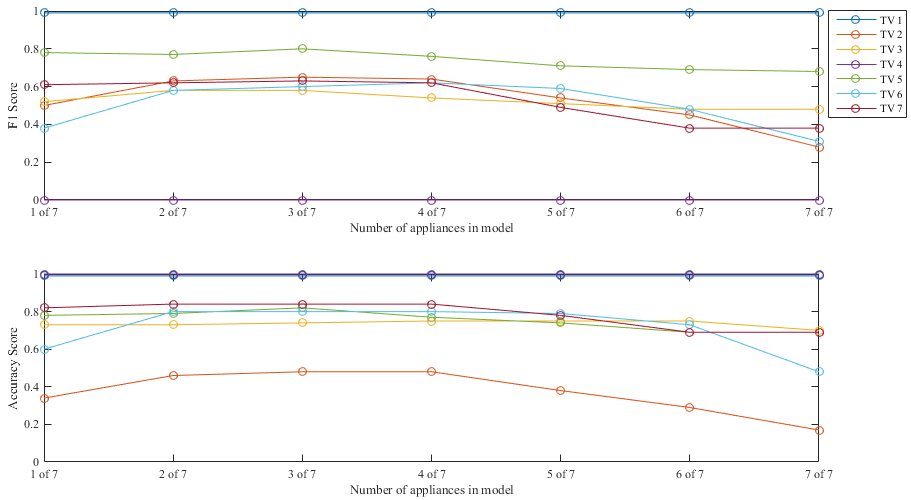
\includegraphics[width=1\textwidth]{billeder/ModelCompletness.png}
\caption{Completeness test of disaggregation of appliances in the TV house dataset }
\label{fig:COD}
\end{figure}

In figure \ref{fig:COD} is the result for each appliance shown. The result is an average of all tests at a given model \df{completeness}. It is seen from the figure that even though the disaggregation algorithm obtains more information about the complete house, it does not improve the recondition. 

This indicates that 7 instances of the algorithms working in parallel, each disaggregating one meter, would obtain the same results as one model capable of seeing the house as a whole. It is worth mentioning that these tests are based on the \ab{FHMM} algorithm and other algorithms might preform different in this aspect. 

The results indicate that the performance is more depended on the \df{complexity} of the model, rather than the \df{completeness}.

\section{Chapter Summery}
The findings in this chapter indicates that the \df{complexity} of a dataset has a profound impact on the detection performance. A simple way to decrease the performance in a house is to look at each phase in the house separately. This is one of the techniques used in the \ab{ECO} dataset to improve the performance in the system. This does require additional knowledge of which appliances that are connected to which phases. This knowledge can be analytically extracted from the dataset, or supplied by the household. 

It is also indicated that the methods based on the \ab{HMM} does not greatly improve by knowing the entire house model, in relation to only knowing a sub part. This can indicate that a system that focus on detecting each appliance individuality, potentially can detect the appliance as well as one that tires to see the house as a whole.   

The many problems that can occur when using small consumers and once that are similar in behaviour is nicely illustrated in the chapter. The \df{appliance interference} effect for similar appliances is greatly decreasing the overall performance. This makes the small consumers almost undetectable. In order to better this performance, more unique features is needed. This could either be higher frequency features, as discussed in Chapter \ref{sec:AppRec}, or by using reactive features. Furthermore it is shown that the best performance is obtained by training in the same environment as the solution will be deployed in. This is a subject that is also discussed by the developers of the Parson and Weiss algorithms~\citep{RefWorks:28},~\citep{RefWorks:23}, where they discussed ways to train or fit the models to the desired deployment environment.  